\documentclass[conference]{IEEEtran}
\IEEEoverridecommandlockouts
% The preceding line is only needed to identify funding in the first footnote. If that is unneeded, please comment it out.
\usepackage{cite}
\usepackage{amsmath,amssymb,amsfonts}
\usepackage{algorithmic}
\usepackage{graphicx}
\usepackage{textcomp}
\usepackage{xcolor}
\usepackage[acronym]{glossaries}
\usepackage{subcaption}


\def\BibTeX{{\rm B\kern-.05em{\sc i\kern-.025em b}\kern-.08em
    T\kern-.1667em\lower.7ex\hbox{E}\kern-.125emX}}
\begin{document}

\title{Object detection for Verification Based Annotation}
\author{\IEEEauthorblockN{Oliver Batchelor\IEEEauthorrefmark{1} and
Richard Green\IEEEauthorrefmark{2}}
\IEEEauthorblockA{Department of Computer Science,
University of Canterbury\\
Christchurch, New Zealand\\
Email: \IEEEauthorrefmark{1}oliver.batchelor@canterbury.ac.nz,
\IEEEauthorrefmark{2}richard.green@canterbury.ac.nz}}


\newacronym{VBA}{VBA}{Verification Based Annotation}
\newacronym{FCN}{FCN}{Fully Convolutional Network}
\newacronym{FPN}{FPN}{Feature Pyramid Network}


\newacronym{IID}{IID}{Independent and Identically Distributed}

\newacronym{IOU}{IoU}{Intersection over Union}
\newacronym{VOC}{VOC}{Visual Object Classes}
\newacronym{mIOU}{mIOU}{mean Intersection Over Union}

\newacronym{mAP}{mAP}{mean Average Precision}
\newacronym{AP}{AP}{Average Precision}


\newacronym{CRF}{CRF}{Conditional Random Field}

\newacronym{RELU}{ReLU}{Rectified Linear Unit}
\newacronym{PRELU}{PReLU}{Parameterised Rectified Linear Unit}
\newacronym{DECAF}{DeCAF}{Deep Convolutional Activation Feature}

\newacronym{FPN}{FPN}{Feature Pyramid Network}


\newacronym{NLL}{NLL}{Negative Loss Likelihood}
\newacronym{BCE}{BCE}{Binary Cross Entropy}
\newacronym{CE}{CE}{Cross Entropy}

\newacronym{EER}{EER}{Equal Error Rate}

 
\newacronym{COCO}{COCO}{Microsoft Common Objects in Context}
\newacronym{ILSVRC}{ILSVRC}{ImageNet Large Scale Visual Recognition Challenge}

\newacronym{NN}{NN}{Neural Network}
\newacronym{DNN}{DNN}{Deep Neural Network}

\newacronym{CNN}{CNN}{Convolutional Neural Network}
\newacronym{MCDNN}{MCDNN}{Multi-Column Deep Neural Network}

\newacronym{SSD}{SSD}{Single Shot Detector}
\newacronym{RCNN}{R-CNN}{Region CNN}

\newacronym{NMS}{NMS}{Non Maxima Suppression}


\newacronym{SIFT}{SIFT}{Scale Invariant Feature Transform}
\newacronym{SURF}{SURF}{Speeded Up Robust Features}

\newacronym{ALOI}{ALOI}{Amsterdam Library of Images}
\newacronym{MSR}{MSR}{Microsoft Research}
\newacronym{AMT}{AMT}{Amazon Mechanical Turk}

\newacronym{BOW}{BoW}{Bag of Words}
\newacronym{BOVW}{BoVW}{Bag of Visual Words}

\newacronym{ANN}{ANN}{Approximate Nearest Neighbour}
\newacronym{SGD}{SGD}{Stochastic Gradient Descent}
\newacronym{ASGD}{ASGD}{Asynchronous Stochastic Gradient Descent}
\newacronym{LOO}{LOO}{Leave One Out}

\newacronym{NCA}{NCA}{Neighbourhood Components Analysis}
\newacronym{MEGM}{MEGM}{Mean square Error's Gradient Minimisation}

\newacronym{KNN}{kNN}{k-Nearest Neighbour}

\newacronym{MSE}{MSE}{Mean Squared Error}
\newacronym{LMNN}{LMNN}{Large Margin Nearest Neighbour}
\newacronym{NCM}{NCM}{Nearest Class Mean}

\newacronym{SVM}{SVM}{Support Vector Machine}

\newacronym{PCA}{PCA}{Principle Components Analysis}
\newacronym{DRLIM}{DrLIM}{Dimensionality Reduction by Learning an Invariant Mapping}
\newacronym{SGDR}{SGDR}{Stochastic Gradient Descent with Restarts}


\newacronym{GPU}{GPU}{Graphics Processing Unit} 
\newacronym{CPU}{CPU}{Central Processing Unit}

\newacronym{API}{API}{Application Programming Interface} 

\newacronym{GHC}{GHC}{Glasgow Haskell Compiler}
\newacronym{GHCJS}{GHCJS}{GHC for JavaScript}

\newacronym{HTML}{HTML}{HyperText Markup Language}
\newacronym{SVG}{SVG}{Scaleable Vector Graphics}

\newacronym{HTTP}{HTTP}{HyperText Transfer Protocol}
\newacronym{JSON}{JSON}{JavaScript Object Notation}

\newacronym{ID}{ID}{Index of Difficulty}
\newacronym{AWS}{AWS}{Amazon Web Services}

\newacronym{CAT}{CAT}{Cumulative Annotation Time}
\newacronym{ROV}{ROV}{Remotely Operated Vehicle}


\maketitle

\begin{abstract}

In this paper we discuss several aspects of an object detector used for the purpose of online training 

\end{abstract}

\begin{IEEEkeywords}
verification, annotation, object detection, neural network, human-in-the-loop
\end{IEEEkeywords}

\section{Introduction}


\subsection{Human-in-the-loop machine learning}

\emph{Human-in-the-loop} machine learning methods are collaborations between a machine learning algorithm and a human user. The goal, where it relates to image annotation, is to make the most effective use of annotator time and reduce cognitive load. Human-in-the-loop approaches can offer improved engagement in activities that would otherwise be laborious.

Machine learning datasets often contain a lot of so-called \emph{easy} examples. These examples often dominate both the annotation process, where human time is spent needlessly annotating similar easy examples, and the learning process where the learning algorithm spends much of its computation time on examples that are already well handled. 

Human-in-the-loop machine learning includes a variety of methods. Examples include Active Learning, where an algorithm asks a human to label only the most uncertain examples, \gls{VBA} using the idea that a human annotator can recognise the correct annotation faster than manually inputting it, and \emph{interactive machine learning} where human input can be used by a machine learning algorithm to direct it, or provide hints. 

\subsection{Verification based annotation}

In this thesis, I use the term Verification Based Annotation (VBA), where machine annotations are checked and verified by a human annotator. Although the idea has played a central role in many previous works, it is not given an easily recognisable term to distinguish it from other kinds of human-in-the-loop machine learning methods such as active learning and is often conflated. A selection of verification based methods are discussed in detail below \cite{Yao2012, McNeill2011, Adhikaria2018, Castrejon2017, Papadopoulos2016, Russakovsky2015a}. 

Verification also plays a large part in ensuring consistency between human annotators in crowdsourcing efforts \cite{Su2012a}. The annotations of any one user cannot be fully trusted, and there can be significant variation between annotators. Often large organisations gamify the annotation process by having users annotate and verify labels as part of a proof-of-human process \cite{von2008recaptcha}.

Weaker algorithms (machine learning or otherwise) can be used to generate proposals which can then be validated by an annotator. An example of this is in \cite{McNeill2011} where computer vision algorithms generate proposed counts of a penguin colony, and a human operator marks false negatives and false positives.

Human verification is fast; in \cite{Papadopoulos2016}, a yes/no verification is reported as taking 1.6 seconds on average. For a full annotation of a \gls{ILSVRC} image, in \cite{Su2012a} the time to draw a bounding box is reported at 26 seconds (42 seconds after quality control), but \cite{Papadopoulos2017} reports only 7 seconds per box using a more effective input method involving clicking extremities of objects rather than selecting corners. 



\section{Method}


\subsection{Datasets}
\begin{figure*}[htbp]
\centering
\begin{subfigure}[t]{0.2\linewidth}
  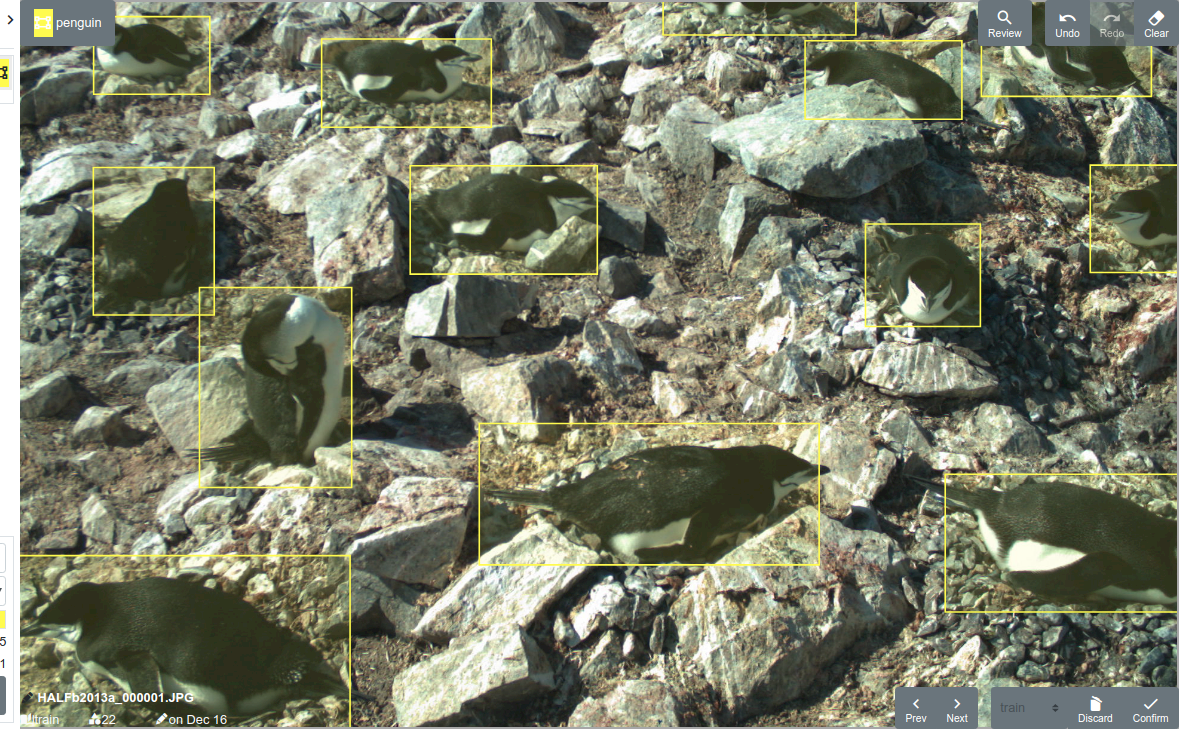
\includegraphics[width=0.9\linewidth]{figures/annotation/screenshots/penguins2.png}
   \caption{\emph{penguins}}
\end{subfigure}%
\begin{subfigure}[t]{0.2\linewidth}
  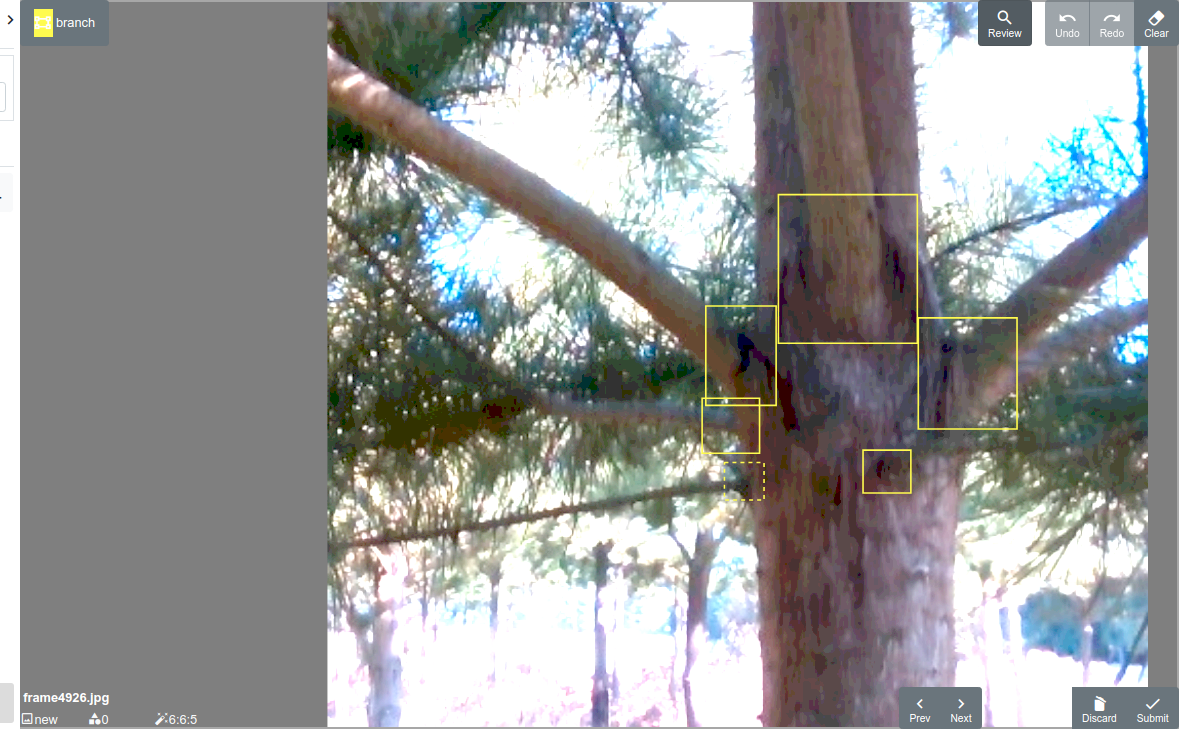
\includegraphics[width=0.9\linewidth]{figures/annotation/screenshots/branches3.png}
   \caption{\emph{branches}}
\end{subfigure}%
\begin{subfigure}[t]{0.2\linewidth}
  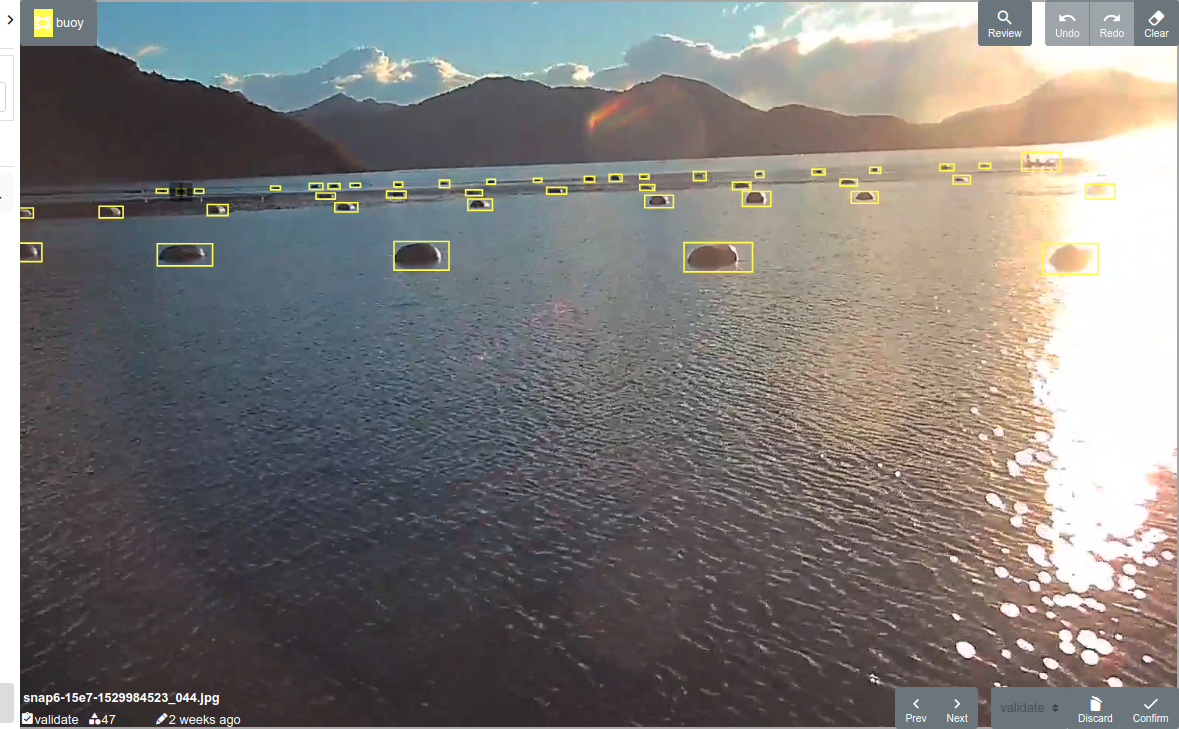
\includegraphics[width=0.9\linewidth]{figures/annotation/screenshots/buoys.png}
   \caption{\emph{buoys}}
 \end{subfigure}%
\begin{subfigure}[t]{0.2\linewidth}
  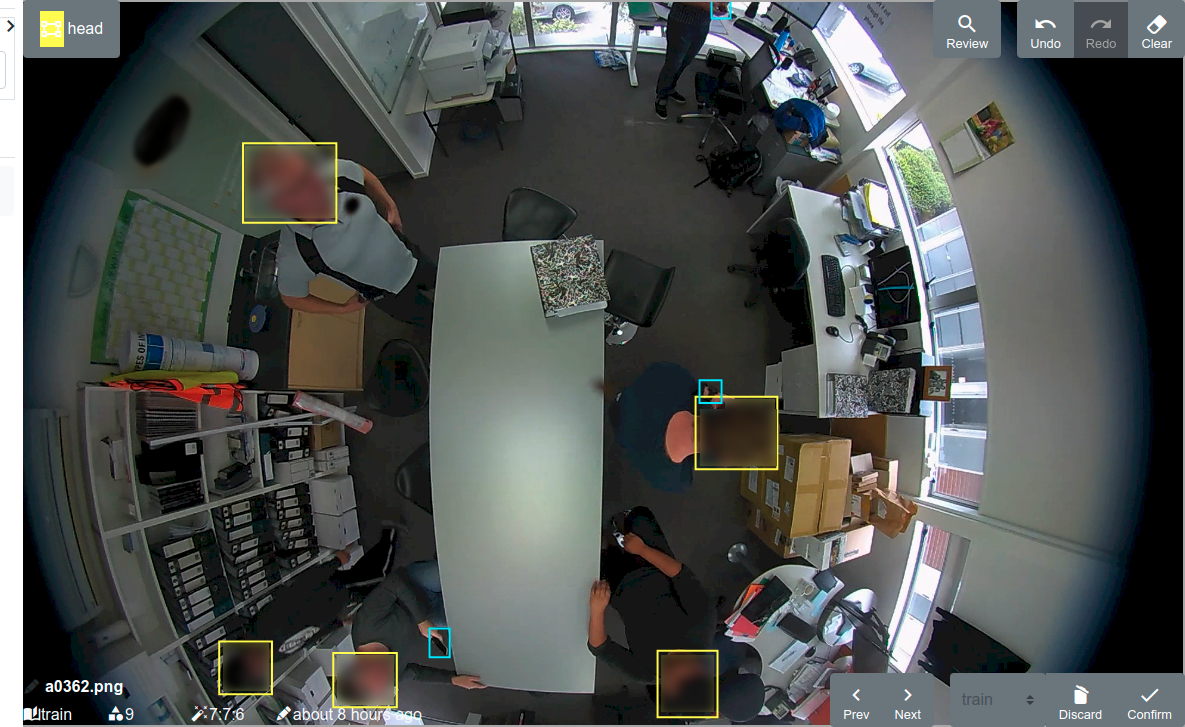
\includegraphics[width=0.9\linewidth]{figures/annotation/screenshots/victor.png}
  \caption{\emph{fisheye}}
\end{subfigure}%
\begin{subfigure}[t]{0.2\linewidth}
  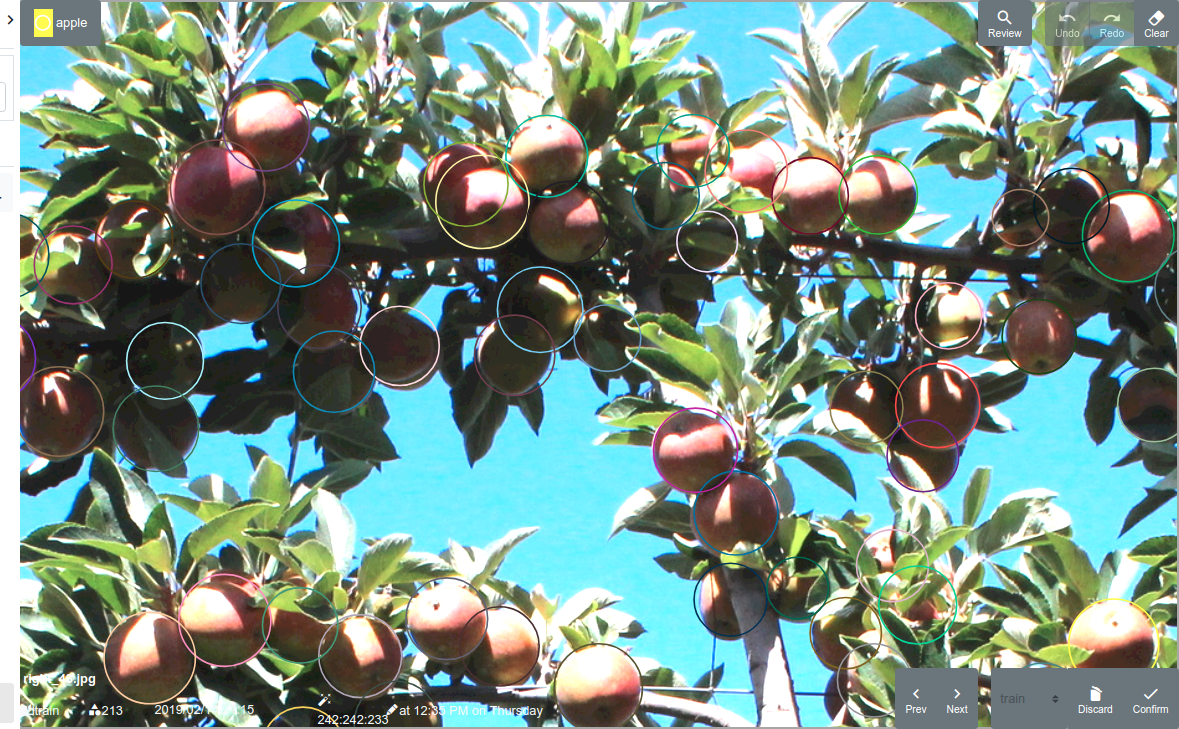
\includegraphics[width=0.9\linewidth]{figures/annotation/screenshots/apples_big2.png}
  \caption{$\mathrm{apples_1}$}
\end{subfigure}
\begin{subfigure}[t]{0.2\linewidth}
  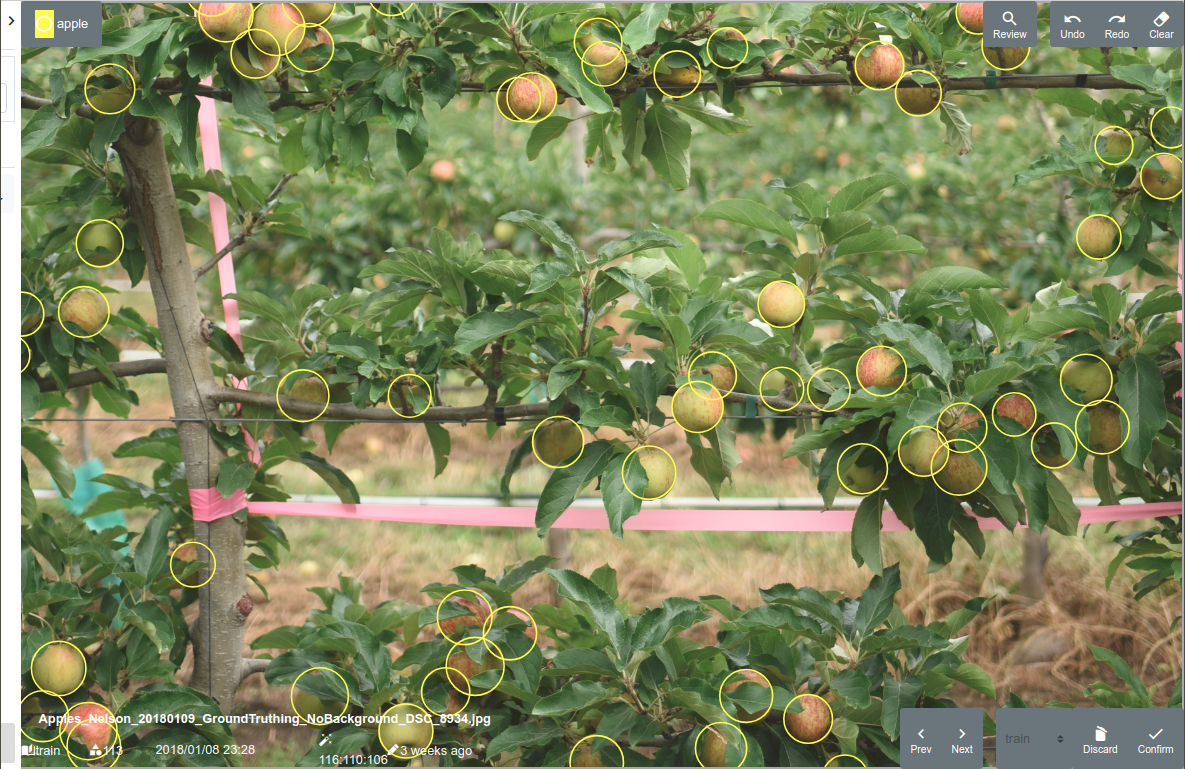
\includegraphics[width=0.9\linewidth]{figures/annotation/screenshots/apples2.png}
  \caption{$\mathrm{apples_2}$}
\end{subfigure}%
 \begin{subfigure}[t]{0.2\linewidth}
  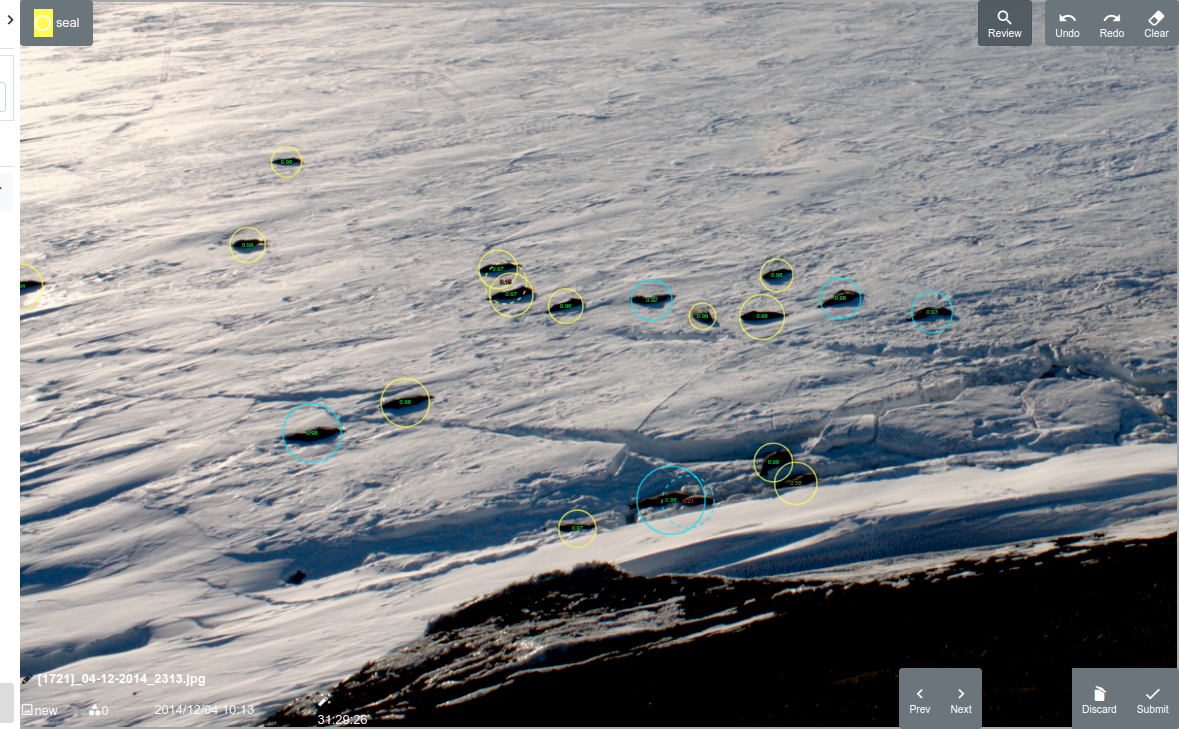
\includegraphics[width=0.9\linewidth]{figures/annotation/screenshots/seals_small2.png}
  \caption{\emph{seals}}
\end{subfigure}%
\begin{subfigure}[t]{0.2\linewidth}
  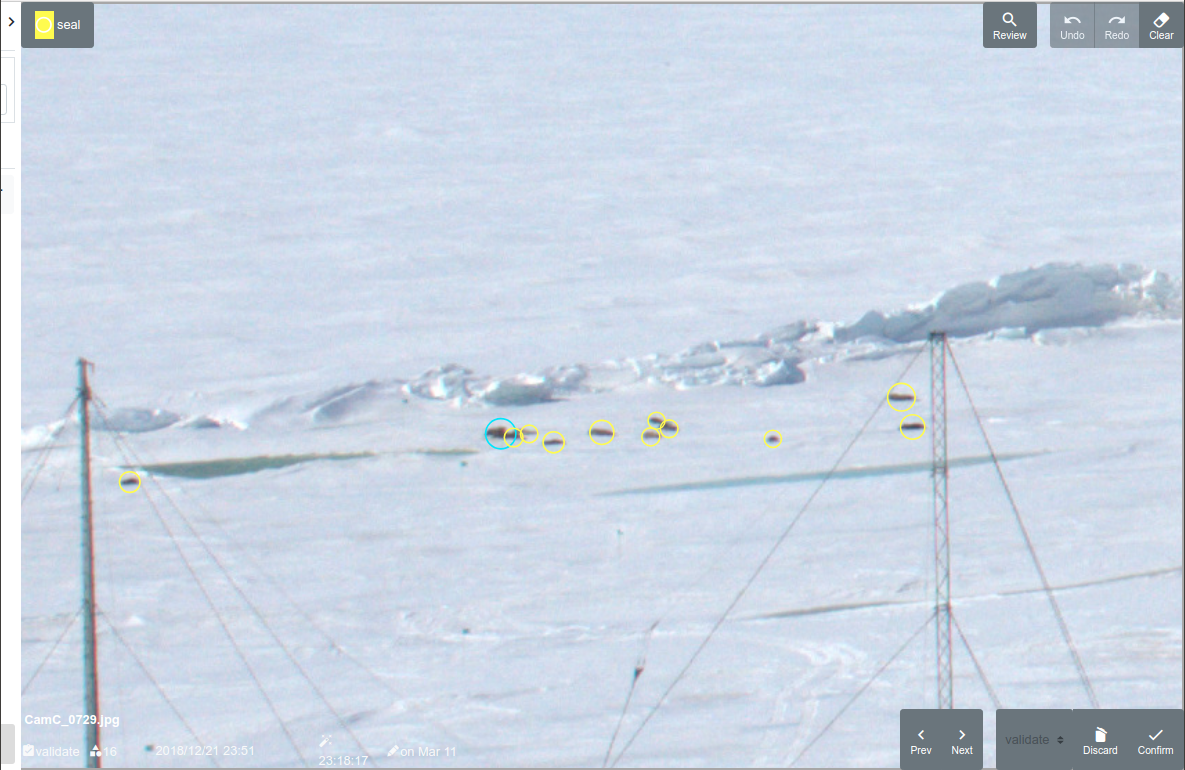
\includegraphics[width=0.9\linewidth]{figures/annotation/screenshots/scott_base_sunny.png}
  \caption{\emph{scott base}}
\end{subfigure}%
\begin{subfigure}[t]{0.2\linewidth}
  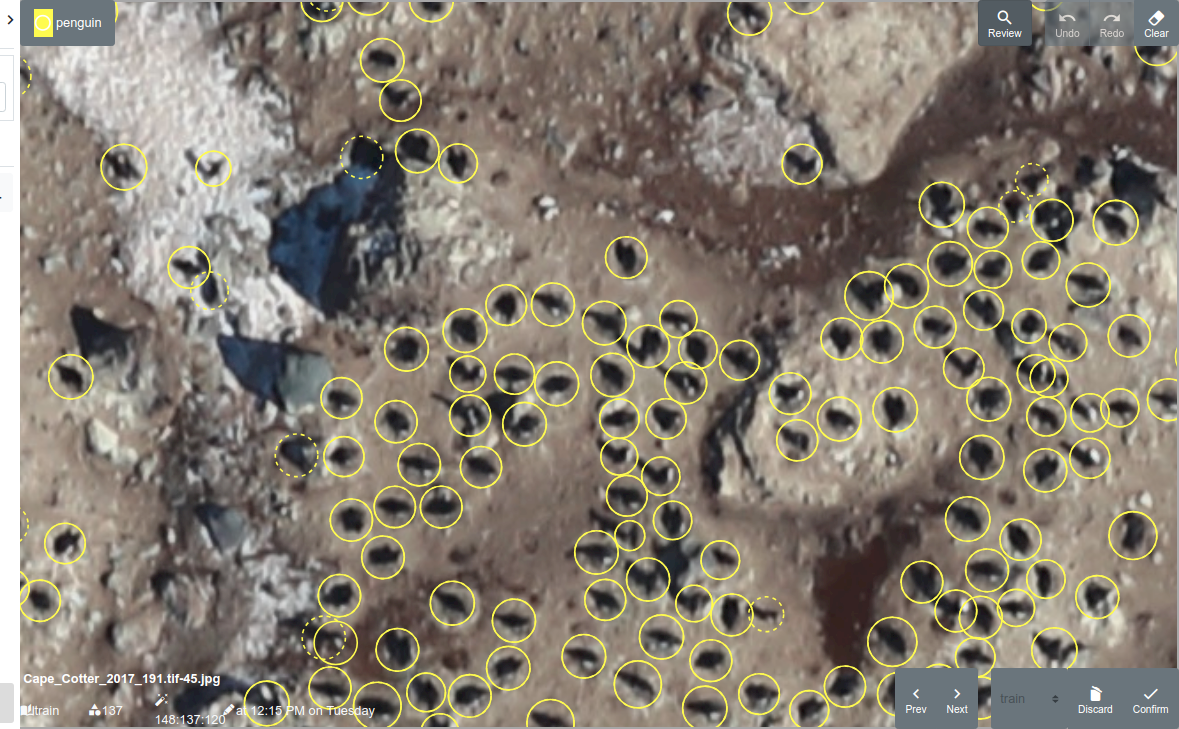
\includegraphics[width=0.9\linewidth]{figures/annotation/screenshots/penguins_aerial2.png}
  \caption{\emph{penguin survey}}
\end{subfigure}%
\begin{subfigure}[t]{0.2\linewidth}
  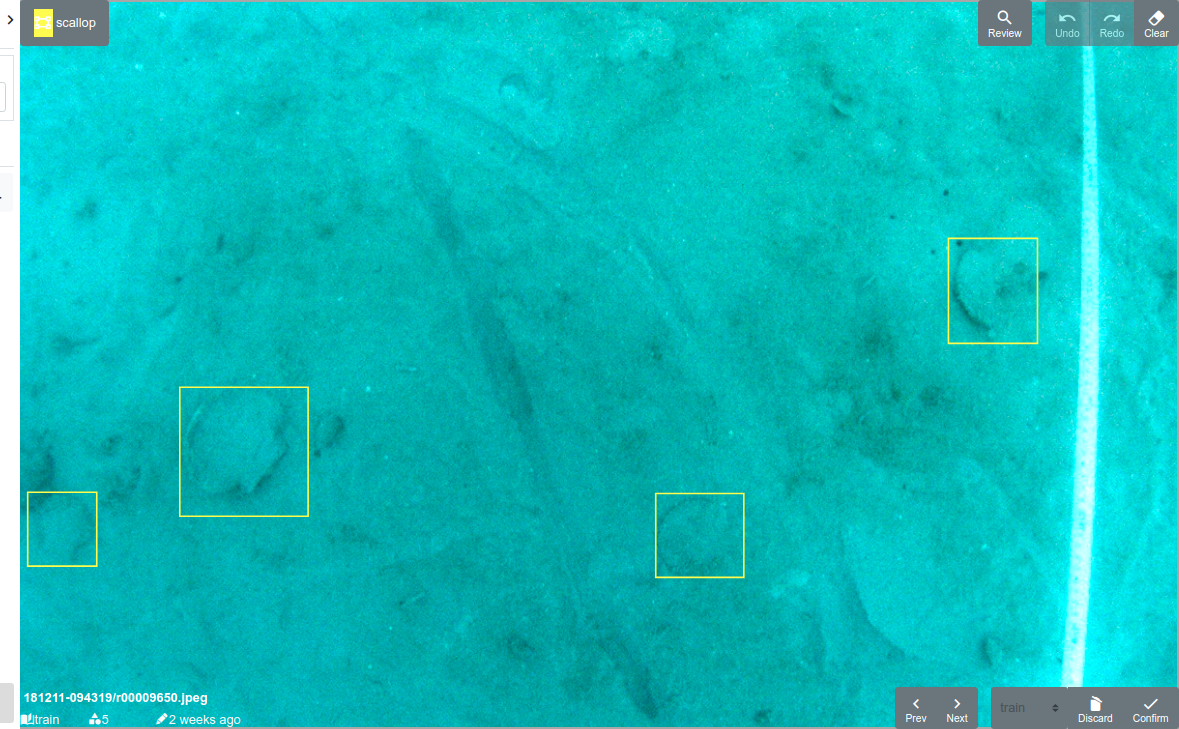
\includegraphics[width=0.9\linewidth]{figures/annotation/screenshots/scallops4.png}
  \caption{\emph{scallops}}
\end{subfigure}
\caption{Representative images of datasets (and annotations) annotated in this work}
\label{fig:datasets_all}
\end{figure*}


\section{High resolution inference}


\section{Effect of localisation noise}



\section*{Acknowledgment}\

\bibliographystyle{unsrt}
\bibliography{references}

\end{document}
